\documentclass[chaptersright]{informeutn}
\usepackage[table]{xcolor}
\usepackage{listings}
\usepackage{pdfpages}
\usepackage{tikz/tikzit}
\usepackage{wrapfig}
\usepackage{ltablex}
\keepXColumns

\input{tikz/TikZiT_style.tikzstyles}

\lstdefinestyle{ltspice}{
  backgroundcolor=\color{gray!10},
  basicstyle=\ttfamily\small,
  keywordstyle=\color{blue},
  commentstyle=\color{green!50!black},
  stringstyle=\color{orange},
  frame=single,
  breaklines=true,
  postbreak=\mbox{\textcolor{red}{$\hookrightarrow$}\space},
  columns=flexible,
  captionpos=b
}
\renewcommand{\lstlistingname}{Listado}

% Datos del informe
\materia{Dispositivos Electrónicos}
\titulo{Trabajo Práctico 5}
\comision{3R2}
\autores{
          Santino Noccetti, 405927 - Operario y Documentador\\
          Franco Palombo, 401910 - Coordinador}
\fecha{04/11/2025}

\begin{document}
  \maketitle

  \tableofcontents
  \setcounter{page}{1}
  \thispagestyle{plain}

  \chapter{Introducción}
  El presente trabajo práctico tiene como objetivo el estudio y análisis de los dispositivos de conmutación
  pertenecientes a la familia de los tiristores, específicamente el Rectificador Controlado de Silicio (SCR), el DIAC y
  el TRIAC. Estos componentes resultan esenciales en el control electrónico de potencia, dado que permiten regular el
  flujo de corriente mediante señales de disparo, posibilitando su aplicación en sistemas de control de iluminación,
  motores, calefactores y circuitos de regulación.

  A lo largo del desarrollo del trabajo se realizaron tanto simulaciones en LTspice como mediciones experimentales en
  laboratorio, con el fin de obtener y comparar las curvas características de cada dispositivo. Se analizaron las
  condiciones de disparo, conducción y apagado, así como los parámetros eléctricos asociados —tales como corriente y
  tensión de compuerta, corriente de mantenimiento y tensión de ruptura—.

  Asimismo, se llevó a cabo la interpretación de hojas de datos de los dispositivos empleados (TYN612M, DB3 y BT136),
  con el propósito de contrastar los valores teóricos provistos por el fabricante con los obtenidos en las experiencias.
  De esta manera, el trabajo permitió consolidar los conocimientos teóricos sobre el comportamiento de los tiristores y
  su respuesta ante diferentes condiciones de operación.

  \chapter{Rectificador Controlado de Silicio}
  \begin{wrapfigure}{R}{0.3\textwidth}
  \vspace{-1cm}
    \centering
    \resizebox{!}{\linewidth}{
    \begin{tikzpicture}
	\begin{pgfonlayer}{nodelayer}
		\node [style=none] (0) at (-1, 2) {};
		\node [style=none] (1) at (1, 2) {};
		\node [style=none] (2) at (-1, 1) {};
		\node [style=none] (3) at (1, 1) {};
		\node [style=none] (4) at (-1, 0) {};
		\node [style=none] (5) at (1, 0) {};
		\node [style=none] (6) at (-1, -1) {};
		\node [style=none] (7) at (1, -1) {};
		\node [style=none] (8) at (-1, -2) {};
		\node [style=none] (9) at (1, -2) {};
		\node [style=none] (10) at (-0.5, -2) {};
		\node [style=none] (11) at (0.5, -2) {};
		\node [style=none] (12) at (-0.5, -2.25) {};
		\node [style=none] (13) at (0.5, -2.25) {};
		\node [style=none] (14) at (-0.5, 2.25) {};
		\node [style=none] (15) at (0.5, 2.25) {};
		\node [style=none] (16) at (-0.5, 2) {};
		\node [style=none] (17) at (0.5, 2) {};
		\node [style=none] (18) at (-1.25, -0.25) {};
		\node [style=none] (19) at (-1, -0.25) {};
		\node [style=none] (20) at (-1.25, -0.75) {};
		\node [style=none] (21) at (-1, -0.75) {};
		\node [style=none] (22) at (-1.25, -0.5) {};
		\node [style=none] (23) at (0, -2.25) {};
		\node [style=none] (24) at (0, 2.25) {};
		\node [style=none] (25) at (0, 3) {};
		\node [style=none] (26) at (-2, -0.5) {};
		\node [style=none] (27) at (0, -3) {};
		\node [style=none] (28) at (0, 1.5) {p};
		\node [style=none] (29) at (0, 0.5) {n};
		\node [style=none] (30) at (0, -0.5) {p};
		\node [style=none] (31) at (0, -1.5) {n};
		\node [style=none] (32) at (0, -3.25) {K};
		\node [style=none] (33) at (0, 3.25) {A};
		\node [style=none] (34) at (-2.25, -0.5) {G};
	\end{pgfonlayer}
	\begin{pgfonlayer}{edgelayer}
		\draw [style=fill2] (3.center)
			 to (2.center)
			 to (0.center)
			 to (1.center)
			 to cycle;
		\draw [style=fill2] (4.center)
			 to (6.center)
			 to (7.center)
			 to (5.center)
			 to cycle;
		\draw [style=fill3] (4.center)
			 to (5.center)
			 to (3.center)
			 to (2.center)
			 to cycle;
		\draw [style=fill3] (8.center)
			 to (9.center)
			 to (7.center)
			 to (6.center)
			 to cycle;
		\draw [style=fill4] (10.center)
			 to (12.center)
			 to (13.center)
			 to (11.center)
			 to cycle;
		\draw [style=fill4] (14.center)
			 to (16.center)
			 to (17.center)
			 to (15.center)
			 to cycle;
		\draw [style=fill4] (18.center)
			 to (20.center)
			 to (21.center)
			 to (19.center)
			 to cycle;
		\draw (22.center) to (26.center);
		\draw (24.center) to (25.center);
		\draw (23.center) to (27.center);
	\end{pgfonlayer}
\end{tikzpicture}

    }
    \caption{estructura interna del SCR.}
    \label{fig:scr_si}
  \end{wrapfigure}
  Un SCR (rectificador controlado de silicio, silicon-controlled rectifier) es un dispositivo pnpn de 4 capas similar al
  diodo de 4 capas pero con tres terminales: ánodo, cátodo y compuerta. En la figura \ref{fig:scr_si} puede ver la
  construcción básica del mismo, y su símbolo esquemático.

  \section{Activación del SCR}
    Cuando la corriente en la compuerta, $I_G$, es cero, por lo que el dispositivo actúa como un diodo de 4 capas en el
    estado de apagado. En este estado, la muy alta resistencia entre el ánodo y el cátodo pueden ser simulados de forma
    aproximada por un interruptor abierto. Cuando se aplica un pulso (disparo) positivo de corriente a la compuerta, el
    dispositivo se enciende, generando un camino de baja resistencia para permitir el flujo de corriente entre ánodo y
    cátodo. El SCR se puede activar también por voltaje entre ánodo y cátodo, ya que mientras que $I_G = 0$, el componente
    se comportara como un diodo de 4 capas.

    Se propuso analizar las regiones de acrivacion y corrientes de codo del SCR seleccionado y compararlas con las
    provistas por el fabricante en el datasheet. Para nuestra practica, seleccionamos el TYN612M. Para analizar las
    diferentes regiones, se realizaran 3 pruebas:
    \begin{itemize}
      \item Curva de $I_G = f_{(V_G)}$ para $V_{AK} = 0V$,
      \item Curva de $I_A = f_{(V_{AK})}$ para $V_G = 0V$,
      \item Curva de $I_A = f_{(V_G)}$ para $V_{AK} = 100V$.
    \end{itemize}

    Por cuestiones de seguridad, la curva de $I_A = f_{(V_{AK})}$ para $V_G = 0V$ solo se realizara en simulación.

    \subsection{Curva $I_G = f_{(V_G)}$}
      Para lograr esta curva, la única condición que se debe aplicar es mantener $V_{AK} = 0V$ en todo momento,
      mientras se varia el $V_G$.

      \subsubsection{Actividad de simulación}
        Se propuso realizar un barrido lineal de la tensión $V_G$ mientras que $V_{AK} = 0V$. El barrido es de $0V$ a
        $20V$ en pasos de $100mV$. Para trazar esta curva, el circuito utilizado es el de la figura \ref{crkt:scr_vak0}
        y los parámetros de simulación se pueden ver en \ref{list:scr_vak0}.
        \begin{figure}[!ht]
          \centering
          \begin{minipage}{0.45\textwidth}
            \centering
            \input{tikz/crkt_scr_vak0.tikz}
            \caption{circuito del SCR a simular}
            \label{crkt:scr_vak0}
          \end{minipage}
          \hfill
          \begin{minipage}{0.45\textwidth}
            \centering
          \begin{lstlisting}[style=ltspice, caption={Parámetros de simulación LTspice}, label=list:scr_vak0]
.dc V1 0 20 100m
          \end{lstlisting}
          \end{minipage}
        \end{figure}

      Revise la sección \ref{annex:scr_model} para ver el modelo SPICE utilizado para las simulaciones.
      \begin{figure}[!ht]
        \begin{tikzpicture}
          \begin{axis}[
            width=14cm,
            height=5.5cm,
            xlabel={$V_G$ [mV]},
            ylabel={$I_G$ [mA]},
            grid=both,
            minor tick num=1,
            scale only axis,
            enlargelimits=false,
              title={$I_G = f_{(V_G)}$},
            extra x ticks={550},
            extra x tick style={
              grid style={red, thick, dashed},
              tick style={red},
              tick label style={red}
             },
            scaled ticks=false,
            restrict x to domain=0:800,
            xmin=0, xmax=800
          ]
          \addplot[
            color=blue,
            mark=none,
            thick,
          ] table[
            col sep=tab,
            header=true,
            x expr=\thisrow{V(vg)}*1000,
            y expr=\thisrow{Ix(U1:G)}*1000
          ] {simulations/ig_vg_vak0.txt};
          \end{axis}
        \end{tikzpicture}
          \caption{gráfica de la corriente de gate en función de la tensión de gate.}
          \label{graph:scr_ig_vg_vak0}
      \end{figure}

      La curva relevada se puede ver en la figura \ref{graph:scr_ig_vg_vak0}, y esta es bastante similar a la curva de
      un diodo, con el cambio de que el potencial en el que empieza a conducir es menor. Esto se debe a que la unión
      presente entre gate y cátodo es, a los ojos del circuito de gate, un simple diodo.

      \subsubsection{Actividad de Laboratorio}
        Para esta actividad, en vez de variar la fuente, esta se mantuvo fija, y usando un potenciómetro fuimos variando
        su resistencia, provocando un cambio en la $V_G$ y la $I_G$. El circuito utilizado se puede ver en la figura
        \ref{crkt:scr_vak0_lab}.

        \begin{figure}[!ht]
          \centering
          \begin{minipage}{0.7\textwidth}
            \centering
            \resizebox{1\textwidth}{!}{
            \begin{tikzpicture}
	% Paths, nodes and wires:
	\draw (0.56, 2.3) to[american resistor, l={$4K7$}] (3.56, 2.3);
	\draw (7.83, 4) to[american resistor, l={$4K7$}] (7.83, 7);
	\draw (7.83, 4) to[empty thyristor, mirror] (7.83, 2);
	\draw (3.56, 2.3) to[qiprobe, l={$I_G$}] (5.56, 2.3);
	\draw (3.56, 2.3) to[qvprobe, l={$V_G$}] (3.56, -0);
	\draw (7.83, 2) to[qiprobe, l={$I_A$}] (7.83, -0);
	\draw (5.56, 2.3) to[normal open switch, l={$SW_1$}] (7.06, 2.3);
	\draw (10.06, 4) to[qvprobe, l_={$V_{AK}$}] (10.06, -0);
	\draw (11.06, 7) to[qvprobe, l={$V_i$}] (11.06, -0);
	\draw (0, 3.925) to[american potentiometer, l_={$5K$}] (0, 0.675);
	\draw (0, 0.675) |- (3.56, -0);
	\draw (3.56, -0) -- (7.83, -0) -- (10.06, -0) -- (11.06, -0);
	\node[vcc](N1) at (0, 7){} node[anchor=south] at (N1.text){$+20V$};
	\node[vcc](N2) at (7.83, 7){} node[anchor=south] at (N2.text){$V_i$};
	\draw (11.06, 7) |- (7.83, 7);
	\draw (10.06, 4) |- (7.83, 4);
	\draw (0, 7) -- (0, 3.925);
	\node[ground] at (7.83, -0){};
\end{tikzpicture}
            }
            \caption{circuito a implementar en el laboratorio.}
            \label{crkt:scr_vak0_lab}
          \end{minipage}
          \hfill
          \begin{minipage}{0.25\textwidth}
            \centering
            \includegraphics[width=0.8\textwidth]{pictures/prot_scr.jpg}
            \caption{circuito implementado en el laboratorio.}
          \end{minipage}
        \end{figure}

        Los datos relevados en el laboratorio se pueden ver en la tabla \ref{tab:scr_vak0_lab} y en la figura
        \ref{graph:scr_ig_vg_vak0_lab}. La curva es muy similar a la del diodo, solo que con un potencial de
        conducción mas bajo que el diodo común de silicio.

        \begin{figure}[!ht]
          \centering
          \begin{minipage}{0.3\textwidth}
            \centering
            \begin{tabular}{c|c}
              $V_G$ & $I_G$ \\ \hline
              0.2     & 0.82     \\
              0.3     & 1.27     \\
              0.4     & 1.73     \\
              0.5     & 2.17     \\
              0.6     & 2.63     \\
              0.7     & 3.79     \\
              0.8     & 5.64     \\
              0.9     &  -       \\
            \end{tabular}
            \caption{datos relevados en el laboratorio}
            \label{tab:scr_vak0_lab}
          \end{minipage}
          \hfill
          \begin{minipage}{0.6\textwidth}
            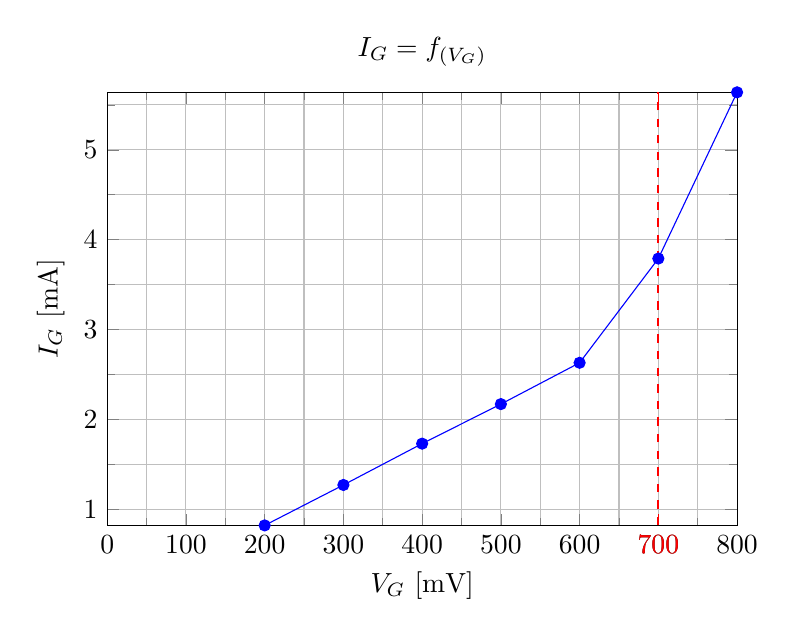
\begin{tikzpicture}
              \begin{axis}[
                width=8cm,
                height=5.5cm,
                xlabel={$V_G$ [mV]},
                ylabel={$I_G$ [mA]},
                grid=both,
                minor tick num=1,
                scale only axis,
                enlargelimits=false,
                  title={$I_G = f_{(V_G)}$},
                extra x ticks={700},
                extra x tick style={
                  grid style={red, thick, dashed},
                  tick style={red},
                  tick label style={red}
                 },
                scaled ticks=false,
                restrict x to domain=0:800,
                xmin=0, xmax=800
              ]
              \addplot[
                color=blue,
                mark=*,
                mark size=2pt,
              ] coordinates {
                (200, 0.82)
                (300, 1.27)
                (400, 1.73)
                (500, 2.17)
                (600, 2.63)
                (700, 3.79)
                (800, 5.64)
              };
              \end{axis}
            \end{tikzpicture}
            \caption{gráfica $I_G = f_{(V_G)}$ relevada en el laboratorio.}
            \label{graph:scr_ig_vg_vak0_lab}
          \end{minipage}
        \end{figure}

      \subsection{Curva $I_A = f_{(V_{AK})}$}
        Para lograr esta curva, la única condición que se debe aplicar es mantener $V_G = 0V$ en todo momento,
        mientras se varia el $V_{AK}$.
          Se propuso realizar un barrido lineal de la tensión $V_{AK}$ mientras que $V_G = 0V$. El barrido es de $0V$ a
          $800V$ en pasos de $10V$. Para trazar esta curva, el circuito utilizado es el de la figura \ref{crkt:scr_vg0}
          y los parámetros de simulación se pueden ver en el listado \ref{list:scr_vg0}.
          \begin{figure}[!ht]
            \centering
            \begin{minipage}{0.45\textwidth}
              \centering
              \input{tikz/crkt_scr_vg0.tikz}
              \caption{circuito del SCR a simular}
              \label{crkt:scr_vg0}
            \end{minipage}
            \hfill
            \begin{minipage}{0.45\textwidth}
              \centering
            \begin{lstlisting}[style=ltspice, caption={Parámetros de simulación LTspice}, label=list:scr_vg0]
.dc V2 0 800 10
            \end{lstlisting}
            \end{minipage}
          \end{figure}

          \begin{figure}[!ht]
            \begin{tikzpicture}
              \begin{axis}[
                width=14cm,
                height=5.5cm,
                xlabel={$V_{AK}$ [V]},
                ylabel={$I_{AK}$ [mA]},
                grid=both,
                minor tick num=1,
                scale only axis,
                enlargelimits=false,
                  title={$I_{AK} = f_{(V_{AK})}$},
                extra x ticks={615},
                extra x tick style={
                  grid style={red, thick, dashed},
                  tick style={red},
                  tick label style={red}
                 },
                extra y ticks={140},
                extra y tick style={
                  grid style={red, thick, dashed},
                  tick style={red},
                  tick label style={red}
                 },
                scaled ticks=false,
                restrict x to domain=0:700,
                xmin=0, xmax=700
              ]
              \addplot[
                color=blue,
                mark=none,
                thick,
              ] table[
                col sep=tab,
                header=true,
                x expr=\thisrow{V(va)},
                y expr=\thisrow{Ix(U1:A)}*1000
              ] {simulations/iak_vak_vg0.txt};
              \end{axis}
            \end{tikzpicture}
              \caption{gráfica de la corriente de ánodo en función de la tensión ánodo-cátodo.}
              \label{graph:scr_iak_vak_vg0}
          \end{figure}

          Como se puede ver en la figura \ref{graph:scr_iak_vak_vg0}, la curva obtenida tiene cierta similitud a la
          curva teórica del SCR y del diodo de 4 capas. Lo que es un poco extraño es la $I_H$, que parece estar
          bastante mas alta que la especificada por la hoja de datos ($20mA$). Esto es muy probablemente una limitacion
          del modelo SPICE.
          %hay que ver de corregir el modelo. La IH es altisima comparada con la de la hoja de datos (approx 20mA)

    \subsection{Curva $I_A = f_{(V_G)}$}
      Para esta curva, se fijara $V_{AK} = 100V$ y haciendo un barrido lineal de $V_G$ trazaremos la curva y
      encontraremos el punto donde el SCR se dispara por corriente de gate.

      \subsubsection{Actividad de Simulación}
        Se propuso realizar un barrido lineal de la tensión $V_g$ mientras que $V_{AK} = 100V$. El barrido es de $0V$ a
        $20V$ en pasos de $100mV$. Para trazar esta curva, el circuito utilizado es el de la figura \ref{crkt:scr_vak100}
        y los parámetros de simulación se pueden ver en \ref{list:scr_vak100}.
        \begin{figure}[!ht]
          \centering
          \begin{minipage}{0.45\textwidth}
            \centering
            \begin{tikzpicture}
	% Paths, nodes and wires:
	\draw (0, 2.3) to[american voltage source, l={$V_1$}] (0, -0);
	\draw (6.77, 4.5) to[american voltage source, l={$V_2$}] (6.77, 2.5);
	\draw (0, 2.3) to[american resistor, l={$4K7$}] (3, 2.3);
	\draw (3.77, 4) to[american resistor, l={$4K7$}] (3.77, 7);
	\draw (3.77, 4) to[empty thyristor, mirror] (3.77, 2);
	\draw (6.77, 4.5) -- (6.77, 7) -- (3.77, 7);
	\draw (3.77, 2) -| (3.77, -0) -- (6.77, -0) -| (6.77, 2.5);
	\draw (0, -0) -- (0.02, -0) -- (3.77, -0);
	\draw (3, 2.3) to[qvprobe, l_={$V_G$}] (3, -0);
	\draw (5.25, 4) to[qvprobe, l={$V_{AK}$}] (5.25, 0);
	\draw (5.25, 4) |- (3.77, 4);
\end{tikzpicture}
            \caption{circuito del SCR a simular}
            \label{crkt:scr_vak100}
          \end{minipage}
          \hfill
          \begin{minipage}{0.45\textwidth}
            \centering
          \begin{lstlisting}[style=ltspice, caption={Parámetros de simulación LTspice}, label=list:scr_vak100]
.dc V1 0 20 100m
          \end{lstlisting}
          \end{minipage}
        \end{figure}

        \begin{figure}[!ht]
          \begin{tikzpicture}
            \begin{axis}[
              width=14cm,
              height=5cm,
              xlabel={$V_G$ [mV]},
              ylabel={$I_{AK}$ [mA]},
              grid=both,
              minor tick num=1,
              scale only axis,
              enlargelimits=false,
                title={$I_{AK} = f_{(V_G)}$},
              scaled ticks=false,
              restrict x to domain=0:700,
              xmin=0, xmax=700
            ]
            \addplot[
              color=blue,
              mark=none,
              thick,
            ] table[
              col sep=tab,
              header=true,
              x expr=\thisrow{V(vg)}*1000,
              y expr=\thisrow{Ix(U1:A)}*1000
            ] {simulations/iak_vg_vak100.txt};
            \end{axis}
          \end{tikzpicture}
            \caption{gráfica de la corriente de ánodo en función de la tensión de gate.}
            \label{graph:scr_iak_vg_vak100}
        \end{figure}

        En la figura \ref{graph:scr_iak_vg_vak100} puede ver el resultado de la simulacion. La cuvra obtenida no se
        parece nada a la teorica. Suponemos que la limitacion se encuentra en el modelo SPICE que no puede modelar el
        comportamiento del SCR en esa region de manera correcta. Existe una amplia variedad de modelos (modelos
        conductuales, modelos equivalentes que utilizan transistores) pero ninguno puede simular el comportamiento de
        todas las regiones del dispositivo real. El mejor modelo que se encontro es el que se esta utilizando, y
        lamentablemente el resultado de la simulacion no es correcto.

        %hay que concluir algo pero el modelo todavia no esta lo suficientemente pulido para generar esta curva de
        %manera adecuada

      \subsubsection{Actividad de Laboratorio}
        Nuevamente, para realizar la variación de la tensión de gate, se hizo lo mismo que para la actividad anterior,
        esto es, dejar fijo el voltaje de gate, y con un potenciómetro ir variando su resistencia y con el su voltaje.
        El circuito empleado es el mismo de la figura \ref{crkt:scr_vak0_lab}.

        Como primer apartado, fijando la $V_{AK} = 100V$ fuimos variando el potenciómetro hasta que notamos que el
        dispositivo se activo por corriente de gate. Los valores relevados son:
        \begin{equation*}
          V_G = 0.8V \quad I_G = 3,31mA
        \end{equation*}

        Posterior a eso, desconectamos el circuito de disparo y notamos que el dispositivo permaneció en la región de
        conducción. Esto es porque la corriente $I_{AK} > I_H$. Posterior a esa prueba, fuimos bajando $V_{AK}$ para
        encontrar cual era la $I_H$ para un $V_G = 0V$. Los datos relevados en el laboratorio se pueden ver en la tabla
        \ref{tab:scr_vak100_lab} y en la figura \ref{graph:scr_ig_vg_vak100_lab}. 

        \begin{figure}[!ht]
          \centering
          \begin{minipage}{0.3\textwidth}
            \centering
            \begin{minipage}{0.45\textwidth}
              \centering
              \begin{tabular}{c|c}
                $V_{AK}$  & $I_{AK}$ \\ \hline
                100       & 20.6      \\
                90        & 18.4      \\
                80        & 16.3      \\
                70        & 14.2      \\
                60        & 12.1      \\
                50        & 9.8       \\
                49        & 9.7       \\
                48        & 9.5       \\
              \end{tabular}
            \end{minipage}
            \hfill
              \begin{minipage}{0.45\textwidth}
              \centering
              \begin{tabular}{c|c}
                $V_{AK}$  & $I_{AK}$ \\ \hline
                47        & 9.3       \\
                46        & 9.1       \\
                45        & 8.9       \\
                44        & 8.7       \\
                43        & 8.5       \\
                42        & 8.3       \\
                41        & 8         \\
                40        & 0         \\
              \end{tabular}
            \end{minipage}
            \caption{datos relevados en el laboratorio}
            \label{tab:scr_vak100_lab}
          \end{minipage}
          \hfill
          \begin{minipage}{0.6\textwidth}
            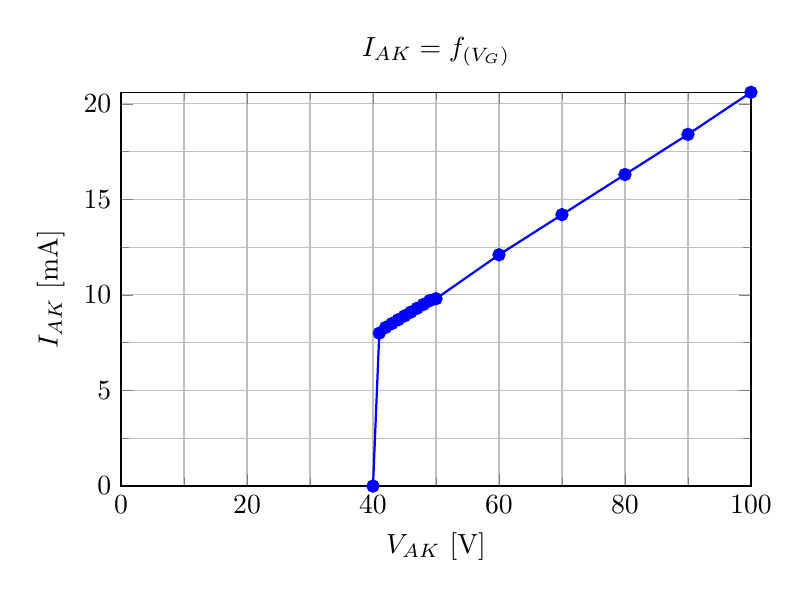
\begin{tikzpicture}
              \begin{axis}[
                width=8cm,
                height=5cm,
                xlabel={$V_{AK}$ [V]},
                ylabel={$I_{AK}$ [mA]},
                grid=both,
                minor tick num=1,
                scale only axis,
                enlargelimits=false,
                  title={$I_{AK} = f_{(V_G)}$},
                extra x ticks={550},
                extra x tick style={
                  grid style={red, thick, dashed},
                  tick style={red},
                  tick label style={red}
                 },
                scaled ticks=false,
                restrict x to domain=0:100,
                xmin=0, xmax=100
              ]
              \addplot[
                color=blue,
                mark=*,
                mark size=2pt,
                thick
              ] coordinates {
                (40, 0.0)
                (41, 8.0)
                (42, 8.3)
                (43, 8.5)
                (44, 8.7)
                (45, 8.9)
                (46, 9.1)
                (47, 9.3)
                (48, 9.5)
                (49, 9.7)
                (50, 9.8)
                (60, 12.1)
                (70, 14.2)
                (80, 16.3)
                (90, 18.4)
                (100, 20.6)
              };
              \end{axis}
            \end{tikzpicture}
            \caption{gráfica $I_{AK} = f_{(V_{AK})}$ relevada en el laboratorio.}
            \label{graph:scr_ig_vg_vak100_lab}
          \end{minipage}
        \end{figure}

        Después de haber logrado apagar el dispositivo haciendo que $I_{AK} < I_H$, procedimos a poner $V_{AK} = 100V$.
        El dispositivo permaneció sin polarización hasta que el circuito de disparo, que quedo con la tensión y
        corriente de disparo, fue conectado, lo que genero que el dispositivo se polarice y comience a circular
        corriente. El comportamiento es idéntico al previamente mencionado.

        Por ultimo, se realizo la prueba de que el SCR quede colocado en inversa, y generar la misma corriente de
        disparo al mismo voltaje. En este caso, no hubo circulación de corriente apreciable, incluso después de subir la
        corriente de gate, por lo que en inversa, el SCR se sigue comportando como un diodo de 4 capas,
        independientemente de la corriente presente en gate.

  \section{Curva característica del SCR}
    Con la información relevada anteriormente respecto a la activación del SCR, podemos ahora pasar a recrear las curvas
    características del SCR. Para ello, la idea es fijar una corriente de gate, e ir haciendo un barrido de la $V_{AK}$
    hasta encontrar el $V_{BR(Fn)}$, voltaje en el cual el dispositivo se polariza y comienza a conducir. El circuito
    implementado en el laboratorio, es el mismo que se utilizo anteriormente. Puede verlo en la figura
    \ref{crkt:scr_curvcar_lab}.

    \begin{figure}[!ht]
      \centering
      \begin{tikzpicture}
	% Paths, nodes and wires:
	\draw (0.56, 2.3) to[american resistor, l={$4K7$}] (3.56, 2.3);
	\draw (7.83, 4) to[american resistor, l={$4K7$}] (7.83, 7);
	\draw (7.83, 4) to[empty thyristor, mirror] (7.83, 2);
	\draw (3.56, 2.3) to[qiprobe, l={$I_G$}] (5.56, 2.3);
	\draw (3.56, 2.3) to[qvprobe, l={$V_G$}] (3.56, -0);
	\draw (7.83, 2) to[qiprobe, l={$I_A$}] (7.83, -0);
	\draw (5.56, 2.3) to[normal open switch, l={$SW_1$}] (7.06, 2.3);
	\draw (10.06, 4) to[qvprobe, l_={$V_{AK}$}] (10.06, -0);
	\draw (11.06, 7) to[qvprobe, l={$V_i$}] (11.06, -0);
	\draw (0, 3.925) to[american potentiometer, l_={$5K$}] (0, 0.675);
	\draw (0, 0.675) |- (3.56, -0);
	\draw (3.56, -0) -- (7.83, -0) -- (10.06, -0) -- (11.06, -0);
	\node[vcc](N1) at (0, 7){} node[anchor=south] at (N1.text){$+20V$};
	\node[vcc](N2) at (7.83, 7){} node[anchor=south] at (N2.text){$V_i$};
	\draw (11.06, 7) |- (7.83, 7);
	\draw (10.06, 4) |- (7.83, 4);
	\draw (0, 7) -- (0, 3.925);
	\node[ground] at (7.83, -0){};
\end{tikzpicture}
      \caption{circuito a implementar en el laboratorio.}
      \label{crkt:scr_curvcar_lab}
    \end{figure}

    \begin{table}[!ht]
      \centering
      \begin{tabular}{c|c|c|c|c|c|c|c|c|c}
        \multicolumn{2}{c|}{$I_G = mA$} & \multicolumn{2}{c|}{$I_G = mA$} & \multicolumn{2}{c|}{$I_G = mA$} & \multicolumn{2}{c|}{$I_G = mA$} & \multicolumn{2}{c}{$I_G = mA$} \\
        $V_{AK}$ & $I_{AK}$ & $V_{AK}$ & $I_{AK}$ & $V_{AK}$ & $I_{AK}$ & $V_{AK}$ & $I_{AK}$ & $V_{AK}$ & $I_{AK}$ \\ \hline
        0 & 2.9 & 0 & 3.05 & 0 & 3.13 & 0 & 3.22 & 0 & 3.22\\
        100 & 2.91 & 80 & 3.05 & 30 & 3.18 & 20 & 3.33 & 5 & 3.39\\
        200 & 2.91 & 80 & 3.05 & 30 & 3.18 & 20 & 3.33 & 5 & 3.39\\
        300 & 2.91 & 240 & 3.06 & 90 & 3.19 & 60 & 3.34 & 15 & 3.4\\
        400 & 2.92 & 300 & 3.07 & 120 & 3.20 & 80 & 3.34 & 20 & 3.4\\
        500 & 2.92 & 400 & 3.08 & 150 & 3.2 & 100 & 3.35 & 25 & 3.4\\
        600 & 2.93 & 480 & 3.09 & 180 & 3.21 & 120 & 3.36 & 30 & 3.41\\
        - & - & - & - & 210 & 3.22 & 140 & 3.37 & 35 & 3.41\\
        - & - & - & - & 240 & 3.22 & 160 & 3.38 & 40 & 3.41\\
        - & - & - & - & 270 & 3.21 & 180 & 3.4 & 45 & 3.41\\
        - & - & - & - & 300 & 3.23 & - & - & 50 & 3.42\\
        - & - & - & - & 330 & 3.26 & - & - & 55 & 3.42\\
        
      \end{tabular}
      \caption{valores relevados en el laboratorio.}
      \label{tab:scr_curvcar_lab}
    \end{table}

    \begin{figure}[!ht]
      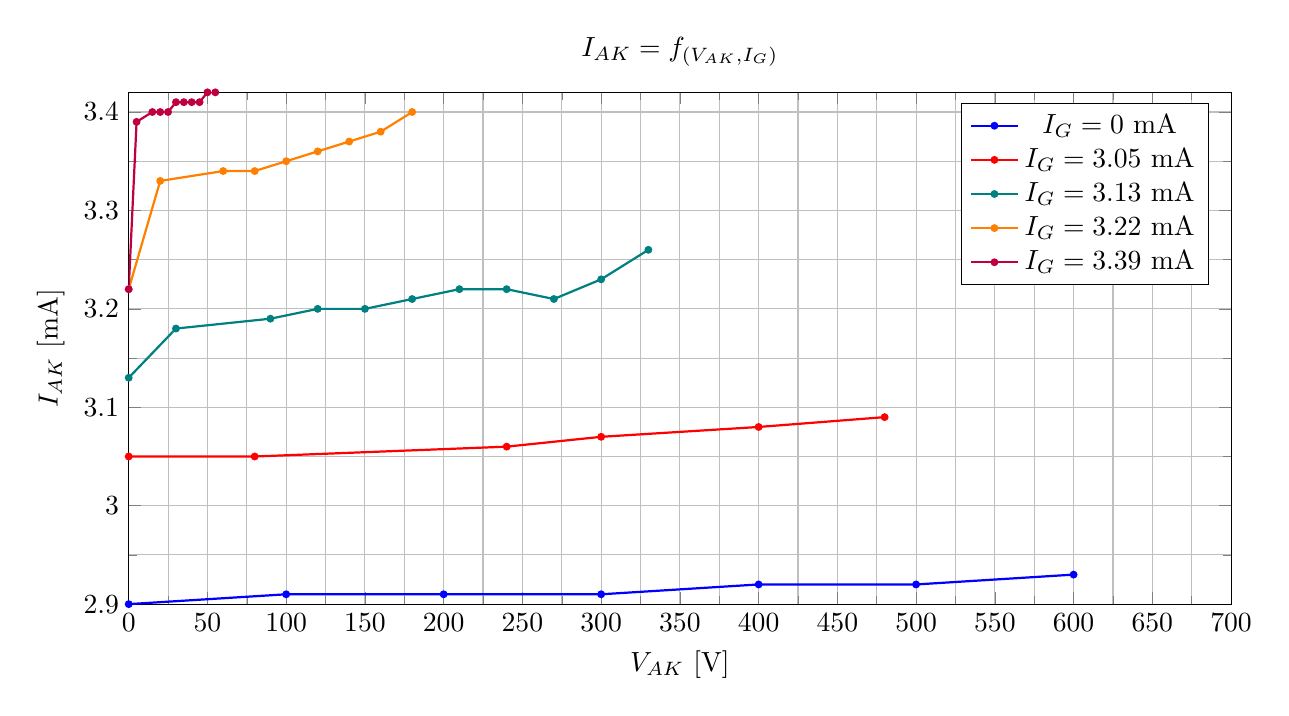
\begin{tikzpicture}
        \begin{axis}[
          width=14cm,
          height=6.5cm,
          xlabel={$V_{AK}$ [V]},
          ylabel={$I_{AK}$ [mA]},
          grid=both,
          minor tick num=1,
          scale only axis,
          enlargelimits=false,
          title={$I_{AK} = f_{(V_{AK}, I_G)}$},
          scaled ticks=false,
          restrict x to domain=0:700,
          xmin=0, xmax=700
        ]
        % --- I_G = 0 mA (columna 1) ---
        \addplot[
          color=blue,
          mark=*,
          mark size=1pt,
          thick
        ] coordinates {
          (0,2.90)
          (100,2.91)
          (200,2.91)
          (300,2.91)
          (400,2.92)
          (500,2.92)
          (600,2.93)
        };
        \addlegendentry{$I_G = 0$ mA}

        % --- I_G = 3.05 mA (columna 2) ---
        \addplot[
          color=red,
          mark=*,
          mark size=1pt,
          thick
        ] coordinates {
          (0,3.05)
          (80,3.05)
          (240,3.06)
          (300,3.07)
          (400,3.08)
          (480,3.09)
        };
        \addlegendentry{$I_G = 3.05$ mA}

        % --- I_G = 3.13 mA (columna 3) ---
        \addplot[
          color=teal,
          mark=*,
          mark size=1pt,
          thick
        ] coordinates {
          (0,3.13)
          (30,3.18)
          (90,3.19)
          (120,3.20)
          (150,3.20)
          (180,3.21)
          (210,3.22)
          (240,3.22)
          (270,3.21)
          (300,3.23)
          (330,3.26)
        };
        \addlegendentry{$I_G = 3.13$ mA}

        % --- I_G = 3.22 mA (columna 4) ---
        \addplot[
          color=orange,
          mark=*,
          mark size=1pt,
          thick
        ] coordinates {
          (0,3.22)
          (20,3.33)
          (60,3.34)
          (80,3.34)
          (100,3.35)
          (120,3.36)
          (140,3.37)
          (160,3.38)
          (180,3.40)
        };
        \addlegendentry{$I_G = 3.22$ mA}

        % --- I_G = 3.39 mA (columna 5) ---
        \addplot[
          color=purple,
          mark=*,
          mark size=1pt,
          thick
        ] coordinates {
          (0,3.22)
          (5,3.39)
          (15,3.40)
          (20,3.40)
          (25,3.40)
          (30,3.41)
          (35,3.41)
          (40,3.41)
          (45,3.41)
          (50,3.42)
          (55,3.42)
        };
        \addlegendentry{$I_G = 3.39$ mA}
      \end{axis}
      \end{tikzpicture}
      \caption{familia de curvas de $I_{AK} = f_{V_{AK}, I_G}$}
      \label{graph:scr_curvcar_lab}
    \end{figure}

    Puede revisar los valores relevados en el laboratorio en la tabla \ref{tab:scr_curvcar_lab} y la familia de curvas
    en la figura \ref{graph:scr_curvcar_lab}. Las tablas terminan cuando en el recorrido de tensión a la próxima
    medición generaba el disparo.

  \section{SCR en Corriente Alterna}
  Una aplicación común de los SCR se encuentra en el control de potencia de ca que varían de intensidad luminosa de
  lámparas, calentadores eléctricos y motores eléctricos. En la figura \ref{crkt:scr_ac} se muestra un circuito de
  control de fase de resistencia variable de media onda. La resistencia conectada al SCR representa la resistencia de la
  carga (por ejemplo, un elemento calefactor o el filamento de una lámpara). El resistor R1 (1K5) limita la corriente y
  variando $p$, se ajusta el nivel de disparo para el SCR. Ajustando $p$ se puede hacer que el SCR se dispare en
  cualquier punto del semiciclo positivo de la forma de onda de ca entre $0^\circ$ y $90^\circ$. Esta actividad se
  realizara en el entorno de simulacion.
  \begin{figure}[!ht]
    \centering
    \begin{minipage}{0.45\textwidth}
      \centering
      \begin{tikzpicture}
	% Paths, nodes and wires:
	\draw (0, 4) to[sinusoidal voltage source, l={$20Vpp$}] (0, 2);
	\draw (2, 6) to[american resistor, l={$\{1K5 + (5k-p)\}$}] (2, 4);
	\draw (2, 3) to[american resistor, l={$\{p\}$}] (2, 1);
	\draw (2, 1) to[capacitor, l={$4.7 \mu F$}] (2, -0);
	\draw (2, 3) to[american resistor, l={$1K$}] (4, 3);
	\draw (4, 3) to[empty diode, l={$D$}] (6, 3);
	\draw (6.77, 4.7) to[empty thyristor, mirror, l={$TN815-800H$}] (6.77, 2.7);
	\draw (2, 4) -| (2, 3);
	\draw (0, 2) -| (0, -0) -- (2, -0);
	\draw (6.77, 2.7) |- (2, -0);
	\draw (6.77, 4.7) to[american resistor, l={$1K$}] (6.75, 6.5);
	\draw (6.75, 6.5) -| (0, 4);
	\draw (2, 6) -| (2, 6.5);
	\node[shape=rectangle, minimum width=0.965cm, minimum height=0.465cm] at (1, 2.5){} node[anchor=center, align=center, text width=0.577cm, inner sep=6pt] at (1, 2.5){$50Hz$};
\end{tikzpicture}
      \caption{circuito del SCR a simular}
      \label{crkt:scr_ac}
    \end{minipage}
    \hfill
    \begin{minipage}{0.45\textwidth}
      \centering
    \begin{lstlisting}[style=ltspice, caption={Parámetros de simulación LTspice}, label=list:scr_ac]
.tran 0 1 .96 1m
.step param p 100 5K 500
.include models/st_standard_sensitive_scr.lib
     \end{lstlisting}
     \end{minipage}
   \end{figure}


  \begin{figure}[!ht]
    \centering
    \begin{minipage}{0.5\textwidth}
      Lamentablemente, el circuito propuesto por el profesor no parece tener efectos significativos en el voltaje o la
      corriente de la carga como deberia. Puede revisar la figura \ref{fig:scr_ac} para ver los efectos de haber
      realizado el barrido del potenciometro. Desconocemos el motivo de por que el circuito no genera cambios
      significativos.
    \end{minipage}
    \hfill
    \begin{minipage}{0.4\textwidth}
      \centering
      \includegraphics[width=1\textwidth]{images/scr_ac.png}
      \caption{resultados de simulacion del recortador de media onda.}
      \label{fig:scr_ac}
    \end{minipage}
  \end{figure}


  \chapter{DIAC}
  \begin{wrapfigure}{R}{0.3\textwidth}
  \vspace{-1cm}
    \centering
    \resizebox{!}{\linewidth}{
    \begin{tikzpicture}
	\begin{pgfonlayer}{nodelayer}
		\node [style=none] (0) at (-1, 1.5) {};
		\node [style=none] (2) at (-1, 0.5) {};
		\node [style=none] (3) at (1, 0.5) {};
		\node [style=none] (4) at (-1, -0.5) {};
		\node [style=none] (5) at (1, -0.5) {};
		\node [style=none] (28) at (0, 1) {p};
		\node [style=none] (29) at (0, 0) {n};
		\node [style=none] (30) at (0, -1) {p};
		\node [style=none] (31) at (1, 2.5) {};
		\node [style=none] (32) at (0, 2.5) {};
		\node [style=none] (33) at (0, 1.5) {};
		\node [style=none] (34) at (-1, 2.5) {};
		\node [style=none] (35) at (1, 0.5) {};
		\node [style=none] (36) at (-1, -2.5) {};
		\node [style=none] (37) at (0, -2.5) {};
		\node [style=none] (38) at (0, -1.5) {};
		\node [style=none] (39) at (1, -2.5) {};
		\node [style=none] (40) at (1, -1.5) {};
		\node [style=none] (41) at (-0.5, 2) {n};
		\node [style=none] (42) at (0.5, -2) {n};
		\node [style=none] (43) at (-0.5, 2.5) {};
		\node [style=none] (44) at (-0.5, 2.75) {};
		\node [style=none] (45) at (0.5, 2.75) {};
		\node [style=none] (46) at (0.5, 2.5) {};
		\node [style=none] (47) at (-0.5, -2.5) {};
		\node [style=none] (48) at (0.5, -2.5) {};
		\node [style=none] (49) at (-0.5, -2.75) {};
		\node [style=none] (50) at (0.5, -2.75) {};
		\node [style=none] (51) at (0, 2.75) {};
		\node [style=none] (52) at (0, 3.25) {};
		\node [style=none] (53) at (0, 3.75) {$A_1$};
		\node [style=none] (54) at (0, -2.75) {};
		\node [style=none] (55) at (0, -3.25) {};
		\node [style=none] (56) at (0, -3.75) {$A_2$};
	\end{pgfonlayer}
	\begin{pgfonlayer}{edgelayer}
		\draw [style=fill2] (3.center) to (2.center);
		\draw [style=fill2] (2.center)
			 to (35.center)
			 to (31.center)
			 to (32.center)
			 to (33.center)
			 to (0.center)
			 to cycle;
		\draw [style=fill2] (5.center) to (4.center);
		\draw [style=fill3] (4.center)
			 to (5.center)
			 to (3.center)
			 to (2.center)
			 to cycle;
		\draw [style=fill2] (4.center)
			 to (36.center)
			 to (37.center)
			 to (38.center)
			 to (40.center)
			 to (5.center)
			 to cycle;
		\draw [style=fill3] (33.center)
			 to (32.center)
			 to (34.center)
			 to (0.center)
			 to cycle;
		\draw [style=fill3] (37.center)
			 to (39.center)
			 to (40.center)
			 to (38.center)
			 to cycle;
		\draw [style=fill4] (44.center)
			 to (45.center)
			 to (46.center)
			 to (43.center)
			 to cycle;
		\draw [style=fill4] (49.center)
			 to (50.center)
			 to (48.center)
			 to (47.center)
			 to cycle;
		\draw (51.center) to (52.center);
		\draw (54.center) to (55.center);
	\end{pgfonlayer}
\end{tikzpicture}

    }
    \caption{estructura interna del DIAC.}
    \label{fig:diac_si}
  \end{wrapfigure}
  Un DIAC es un dispositivo semiconductor de cuatro capas y dos terminales (tiristor) que conduce corriente en una u
  otra dirección cuando se activa. La construcción básica de un DIAC se muestran en la figura \ref{fig:scr_si}. Observe
  las dos terminales, designadas A1 y A2. Las capas superior e inferior contienen tanto materiales n como p. El lado
  derecho de la pila se considera como una estructura pnpn con las mismas características de un diodo de cuatro capas,
  mientras que el lado izquierdo es un diodo de cuatro capas invertido que tiene una estructura npnp.

  La conducción ocurre en un DIAC cuando se alcanza el voltaje de ruptura con una u otra polaridad a través de las dos
  terminales. Una vez que se presenta la ruptura, la corriente fluye en una dirección según la polaridad del voltaje a
  través de las terminales. El dispositivo se apaga cuando la corriente se reduce por debajo del valor de retención.

  \section{Reversibilidad del DIAC}
    Para esta actividad de laboratorio, se propuso variar la tensión de alimentación de 0 a 50V, en pasos de 5V, e ir
    midiendo la corriente que circula por el circuito. Una vez completada la prueba, se debe invertir la polaridad del
    circuito y realizar las mismas mediciones. El circuito implementado en el laboratorio se puede ver en la figura
    \ref{crkt:diac_lab}.

    \begin{figure}[!ht]
      \centering
      \begin{minipage}{0.5\textwidth}
        \centering
        \begin{tikzpicture}
	% Paths, nodes and wires:
	\draw (0, 3.5) to[empty bidirectionaldiode] (0, 1.75);
	\draw (0, 3.5) to[american resistor, l={$R_1$}] (0, 5.5);
	\draw (-0, 1.75) to[qiprobe, l={$I_A$}] (-0, -0);
	\draw (2, 3.5) to[qvprobe, l={$V_A$}] (2, -0);
	\draw (4, 5.5) to[qvprobe, l={$V$}] (4, -0);
	\draw (2, 3.5) -- (0, 3.5);
	\draw (4, 5.5) |- (0, 5.5);
	\draw (0, -0) -- (2, -0);
	\draw (2, -0) -- (4, -0);
	\draw (6, 5.5) to[american voltage source, l={$V_i$}] (6, -0);
	\draw (6, -0) -- (4, -0);
	\draw (6, 5.5) |- (4, 5.5);
\end{tikzpicture}
        \caption{circuito DIAC a implementar en el laboratorio.}
        \label{crkt:diac_lab}
      \end{minipage}
      \hfill
      \begin{minipage}{0.4\textwidth}
        \centering
          \includegraphics[width=0.4\textwidth]{pictures/prot_diac.jpg}
        \caption{circuito DIAC implementado en el laboratorio.}
      \end{minipage}
    \end{figure}

    
    \begin{figure}[!ht]
      \centering
      \begin{tabular}{c|cccccccccccccccc}
      $V_i[V]$     & 0  & 30 & 33 & 35 & 37 & 39 & 41 & 43 & 45 & 47 & 49 & 50 \\ \hline
      $V_A[V]$     & 0  & 30 & 29 & 29 & 29 & 29 & 23 & 23 & 23 & 23 & 23 & 23 \\ \hline
      $I_{AK}[mA]$ & 0  & 0  & 1.73 & 2.73 & 2.75 & 3.12 & 3.6 & 4.13 & 4.66 & 5.02 & 5.48 & 5.67 \\
      \end{tabular}
      \caption{datos relevados en el laboratorio}
      \label{tab:diac}
    \end{figure}

    \begin{figure}[!ht]
      \centering
      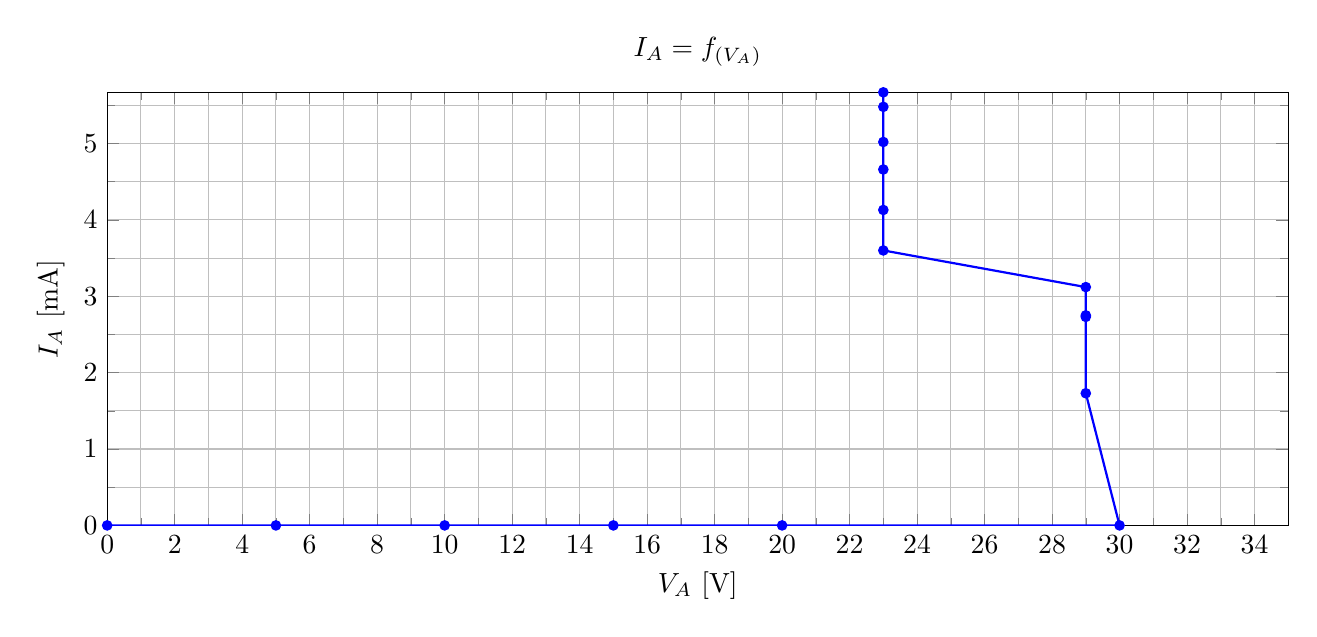
\begin{tikzpicture}
        \begin{axis}[
          width=15cm,
          height=5.5cm,
          xlabel={$V_{A}$ [V]},
          ylabel={$I_{A}$ [mA]},
          grid=both,
          minor tick num=1,
          scale only axis,
          enlargelimits=false,
            title={$I_{A} = f_{(V_A)}$},
          extra x tick style={
            grid style={red, thick, dashed},
            tick style={red},
            tick label style={red}
           },
          scaled ticks=false,
          restrict x to domain=0:35,
          xmin=0, xmax=35
        ]
        \addplot[
          color=blue,
          mark=*,
          mark size=1.5pt,
          thick
        ] coordinates {
          (0,0)
          (5,0)
          (10,0)
          (15,0)
          (20,0)
          (30,0)
          (29,1.73)
          (29,2.73)
          (29,2.75)
          (29,3.12)
          (23,3.6)
          (23,4.13)
          (23,4.66)
          (23,5.02)
          (23,5.48)
          (23,5.67)
        };
        \end{axis}
      \end{tikzpicture}
      \caption{gráfica $I_A = f_{(V_A)}$ relevada en el laboratorio.}
      \label{graph:diac}
    \end{figure}

    Como puede ver en la figura \ref{graph:diac}, la curva relevada en el laboratorio tiene cierta semejanza a la
    teórica del DIAC. Se puede apreciar que al rededor de $V_A = 30V$ empieza a haber una circulación de corriente, por
    lo que podemos decir que el $V_{BR(F)}$ del DIAC seleccionado esta cerca de los 30V. A medida que continuamos
    subiendo el voltaje, la corriente también fue subiendo, con una disminución del voltaje $V_A$ entre los pines del
    DIAC. En particular, este DIAC tiene una $I_H$ considerablemente grande para el voltaje máximo de operación, por lo
    que la curva no presenta esa disminución prácticamente instantánea de $V_A$ tan característica de los tiristores
    cuando comienza a conducir corriente.

  \chapter{TRIAC}

  \section{Curva característica del TRIAC}

  \section{Recortador de onda con TRIAC}

  \chapter{Interpretación de hojas de datos}
  \textbf{Objetivo:} Interpretar y familiarizarse con los parámetros de los tiristores según las especificaciones del fabricante (\textit{datasheet}).
  
  \section{DIAC DB3}
  \begin{table}[!ht]
    \centering
    \begin{tabular}{l|c|p{8cm}}
      \textbf{Parámetro} & \textbf{Símbolo} & \textbf{Descripción / Significado} \\ \hline
      Tensión de disparo & $V_{BO}$ & Voltaje mínimo necesario para que el DIAC comience a conducir corriente. \\ \hline
      Corriente de disparo & $I_{BO}$ & Corriente correspondiente al punto de ruptura, donde el DIAC pasa al estado conductor. \\ \hline
      Variación de tensión & $\Delta V$ & Caída de tensión que ocurre al pasar del estado de bloqueo al de conducción. \\ \hline
      Corriente de conducción & $I_C$ & Corriente que circula a través del DIAC una vez disparado. \\
    \end{tabular}
    \caption{Parámetros característicos del DIAC DB3.}
  \end{table}
  
  \section{SCR C106}
    \begin{tabularx}{\textwidth}{p{4cm}|c|p{8cm}}
      \textbf{Parámetro} & \textbf{Símbolo} & \textbf{Descripción / Significado} \\ \hline
      Tensión de bloqueo directa/inversa repetitiva & $V_{DRM}$ / $V_{RRM}$ & Máxima tensión que el SCR puede soportar en estado bloqueado (sin conducir). \\ \hline
      Corriente RMS & $I_{T(RMS)}$ & Corriente eficaz máxima permitida a través del SCR en conducción continua. \\ \hline
      Corriente promedio & $I_{T(AV)}$ & Corriente promedio máxima permitida en conducción continua. \\ \hline
      Corriente de sobrecarga instantánea & $I_{TSM}$ & Corriente máxima que puede soportar el SCR durante un pulso corto (no repetitivo). \\ \hline
      Corriente de fuga directa/inversa & $I_{DRM}$ / $I_{RRM}$ & Corriente que circula cuando el SCR está en estado bloqueado. \\ \hline
      Corriente de compuerta & $I_{GT}$ & Corriente mínima en la compuerta necesaria para disparar el SCR. \\ \hline
      Tensión de compuerta & $V_{GT}$ & Tensión necesaria entre compuerta y cátodo para disparo. \\ \hline
      Corriente de mantenimiento & $I_H$ & Corriente mínima que debe circular para mantener el SCR en conducción. \\ \hline
      Tiempo de encendido & $t_{gt}$ & Tiempo entre la aplicación del pulso de compuerta y la conducción total del SCR. \\ \hline
      Tiempo de recuperación & $t_q$ & Tiempo necesario para que el SCR vuelva a su estado de bloqueo después de conducir. \\ \hline
      Resistencia térmica unión-carcasa & $R_{\theta JC}$ & Resistencia térmica entre la unión y la carcasa del dispositivo. \\ \hline
      Resistencia térmica unión-ambiente & $R_{\theta JA}$ & Resistencia térmica entre la unión y el ambiente. \\
      \caption{Parámetros característicos del SCR C106.}
    \end{tabularx}
  
  \section{TRIAC BT136}
    \begin{tabularx}{\textwidth}{p{4cm}|c|p{8cm}}
      \textbf{Parámetro} & \textbf{Símbolo} & \textbf{Descripción / Significado} \\ \hline
      Tensión de bloqueo directa/inversa repetitiva & $V_{DRM}$ / $V_{RRM}$ & Máxima tensión soportada en estado bloqueado. \\ \hline
      Corriente RMS & $I_{T(RMS)}$ & Corriente eficaz máxima en conducción continua. \\ \hline
      Corriente de sobrecarga instantánea & $I_{TSM}$ & Corriente máxima que soporta en un pulso corto no repetitivo. \\ \hline
      Corriente de compuerta & $I_{GT}$ & Corriente mínima requerida en la compuerta para disparo. \\ \hline
      Tensión de compuerta & $V_{GT}$ & Tensión entre compuerta y terminal principal para activar el TRIAC. \\ \hline
      Corriente de mantenimiento & $I_H$ & Corriente mínima necesaria para mantener la conducción. \\ \hline
      Tensión en conducción & $V_T$ & Caída de tensión entre terminales principales durante conducción. \\ \hline
      Tiempo de encendido & $t_{gt}$ & Tiempo necesario desde la señal de compuerta hasta conducción completa. \\ \hline
      Tiempo de recuperación & $t_q$ & Tiempo necesario para volver al estado de bloqueo después de conducción. \\ \hline
      Resistencia térmica unión-carcasa & $R_{\text{th j-mb}}$ & Resistencia térmica entre la unión y la base metálica. \\ \hline
      Resistencia térmica unión-ambiente & $R_{\text{th j-a}}$ & Resistencia térmica entre la unión y el ambiente. \\ \hline
      Temperatura de almacenamiento & $T_{STG}$ & Rango de temperatura segura para almacenamiento. \\ \hline
      Temperatura de operación & $T_J$ & Temperatura máxima de operación de la unión. \\
      \caption{Parámetros característicos del TRIAC BT136.}
    \end{tabularx}

  \chapter{Conclusiones}
  El estudio realizado permitió comprender el principio de funcionamiento y las características esenciales de los
  tiristores, verificando experimentalmente los fenómenos de disparo y conducción que los definen.

  En el caso del SCR, se comprobó su activación mediante corriente de compuerta, así como la presencia de una corriente
  de mantenimiento necesaria para sostener el estado de conducción. El DIAC demostró un comportamiento bidireccional con
  un voltaje de ruptura próximo a los 30 V, mientras que el TRIAC evidenció su capacidad de conducir corriente en ambos
  sentidos, actuando funcionalmente como dos SCR conectados en antiparalelo.

  Las simulaciones y mediciones realizadas presentaron una buena correlación con las curvas teóricas, salvo ciertas
  discrepancias atribuibles a las limitaciones de los modelos SPICE utilizados. En conjunto, el trabajo permitió
  afianzar los conceptos fundamentales de los dispositivos de conmutación controlada, su modelado, y su aplicabilidad en
  circuitos de control de potencia en corriente alterna.

  \chapter{Anexos}
  \section{Rubrica}
\begin{figure}[!h]
  \centering
  \begin{tabular}[c]{|c|c|c|}
    \rowcolor{gray!30}
    \hline
    \textbf{Tarea}                      & \textbf{Puntuación} & \textbf{Máximo}\\
    \hline
    Presentación del informe            &                     & 30\%\\
    \hline
    Explicación del proceso de medición &                     & 40\%\\
    \hline
    Defensa de las conclusiones         &                     & 30\%\\
    \hline
    \textbf{Total}                      &                     & \textbf{100\%}\\
    \hline
  \end{tabular}
\end{figure}

\section{Planilla de Seguimiento}
\begin{figure}[!h]
  \begin{footnotesize}
    \begin{tabular}{|m{1cm}|m{1cm}|m{1.3cm}|m{2cm}|m{1.7cm}|m{1.7cm}|m{1.7cm}|m{1.7cm}|m{1.7cm}|}
      \hline
      Versión del TP & Fecha de Inicio & Revisado Por & Resumen Observaciones Correcciones &
      Fecha de retroalimentación enviada & Cambios realizados por JTP? & Nueva fecha de entrega &
      Aprobado por jefe de cátedra?\\
      \hline
      1.0 (2025) & & & & & & &\\
      \hline
    \end{tabular}
  \end{footnotesize}
\end{figure}
 

  \section{Modelos SPICE}
    \lstinputlisting[style=ltspice, caption={Modelo SPICE del TYN612M},
    label=annex:scr_model]{simulations/models/tny612m.lib}
 
  \section{Hojas de Datos}
    \includepdf[pages=1]{annex/bt137x.pdf}
    \includepdf[pages=2]{annex/db3.pdf}
    \includepdf[pages=1]{annex/tyn612m.pdf}


\end{document}
